\section{实验4:AI基于产品描述生成高低水平个性化广告的能力}

实验3验证了AI在中性广告基础上,针对高水平和低水平人格特质生成个性化广告的能力,结果显示在开放性、外倾性和宜人性三个维度上,AI能够有效生成符合不同人格特质水平的个性化广告。然而,在尽责性维度上,并未观察到显著的匹配效应,这可能与尽责性特质的内在特性有关,或与现有中性广告的基础信息不足,难以准确区分高低尽责性的偏好有关。

尽管实验3证明了AI在已有中性广告基础上调整生成个性化广告的能力,但实际广告创作中,尤其是针对新品或特定市场推广场景,往往缺乏现成的中性广告作为基础。在这些情境下,品牌通常需要基于产品描述直接创作广告内容。因此,实验4旨在进一步探讨AI是否能够基于产品描述直接生成针对不同人格特质的个性化广告,从而验证其在更复杂应用场景下的个性化生成能力。

此外,相较于实验3基于已有广告的微调生成,实验4的任务要求更高,AI不仅需要理解产品描述的核心信息,还需要准确提取与目标人格特质相关的要素,进而生成符合特定人格偏好的广告内容。因此,实验4的研究将进一步扩展AI生成个性化广告的适用范围,验证其生成高效个性化广告的能力。

\subsection{方法}


\textbf{(1)被试}

通过见数平台发布实验,368名参与者自愿参加这项研究。48名参与者由于注意检查测试未通过被剔除,剩余\textbf{320名有效参与者}(年龄范围= 18-57岁;\textit{M}=25.88岁;\textit{SD}=6.30;女性198名)。参与任务的每名参与者获得1元人民币作为报酬。注意力检测包含两部分,分别嵌入在因变量测量和人格问卷中,以明确指令题形式呈现(如“请选2”)。参与者需在两道注意力检测题中均作答正确,方可被纳入有效数据样本。每名被试会随机分配到四个特质(开放性、尽责性、外倾性、宜人性)的条件之一,最终每个特质条件均有约80名被试参与。


\textbf{(2)实验材料:广告设计}

实验材料生成数量与实验3一致,共设计\textbf{2(水平:高/低)* 4(特质:开放性、尽责性、外倾性、宜人性)共8则个性化广告}。与实验3不同,实验4中的个性化广告不是基于现有的中性广告进行调整,而是直接基于产品描述生成。我们选择了与实验3相同的产品,即华为Mate70,为了确保生成内容的真实性与关联性,我们从百度搜索中找到的第一篇华为Mate70亮点介绍网页中提取了主要产品特性作为输入内容。针对每个特质与水平的组合,我们使用GPT4生成个性化广告文案。生成过程基于一套结构化提示词(详见附录),包含任务目标、产品描述、调整与优化要求、策略说明。具体而言,GPT的任务是根据输入的产品描述,结合高/低水平的目标人格特质,生成针对目标消费者的个性化广告文案(详见附录)。

为验证生成的个性化广告是否能够有效传达针对目标消费者的特质,本研究在正式实验前通过见数平台发布了预实验,共有90名参与者自愿参加,并获得1元人民币作为报酬。每名参与者需阅读8则广告,并从2(水平)* 5(特质描述)中选择出最匹配的目标消费者。预实验结果表明,大多数参与者能够正确识别出广告所针对的人格特质,这表明GPT基于产品描述生成的个性化广告在针对特定人格特质的目标消费者设计上具有有效性。


\textbf{(3)问卷测量}

同实验3(详见\ref{study1-substudy3-measures},分别测量广告说服效果和大五人格量表。


\subsection{实验流程}
本实验流程分为两个部分。第一部分,参与者依次阅读每组广告,其中每组广告包含高水平与低水平的个性化广告(例如,针对高外倾性和低外倾性设计的广告),并对每组广告的相对说服效果进行评分。第二部分,参与者完成与人格测试相关的问卷,随后填写包括年龄、性别等在内的人口统计学信息。

\subsection{结果}
我们分别对每个特质的结果进行了回归分析。回归模型的自变量为参与者对应人格特质的得分(尽责性、开放性、外倾性、宜人性),因变量为广告的说服效果。由于评分为二极分布,我们对数据进行了转换,使得得分越高表示相较于低水平个性化广告,参与者对高水平个性化广告的偏好越强。在这一模型中,如果存在匹配效应(即高水平特质的参与者更偏好针对高水平设计的个性化广告,而低水平特质的参与者更偏好针对低水平设计的个性化广告),则回归系数应为正且显著。

结果如图\ref{fig:Study1-exp3-result}所示,展示了针对四种人格特质设计的广告组的标准化效应及其95\%置信区间。结果显示,仅在开放性(\textit{$\beta$} = 1.896,\textit{p} < 0.01)和外倾性(\textit{$\beta$} = 2.366,\textit{p} < 0.001)维度上观察到显著的个性化效果,即高开放性和高外倾性的个体更偏好针对高水平特质设计的广告,而低开放性和低外倾性的个体则更偏好针对低水平特质设计的广告。在宜人性维度(\textit{$\beta$} = 0.687,\textit{p} = 0.490)上,未发现显著的个性化效果,表明高低宜人性个体在广告偏好上无明显差异。值得注意的是,在尽责性维度上,回归结果呈现出负向的个性化效果(\textit{$\beta$} = -1.721,\textit{p} < 0.05),即高尽责性个体更偏好针对低尽责性设计的广告,而低尽责性个体则更偏好针对高尽责性设计的广告。

\begin{figure}[H]
    \centering
    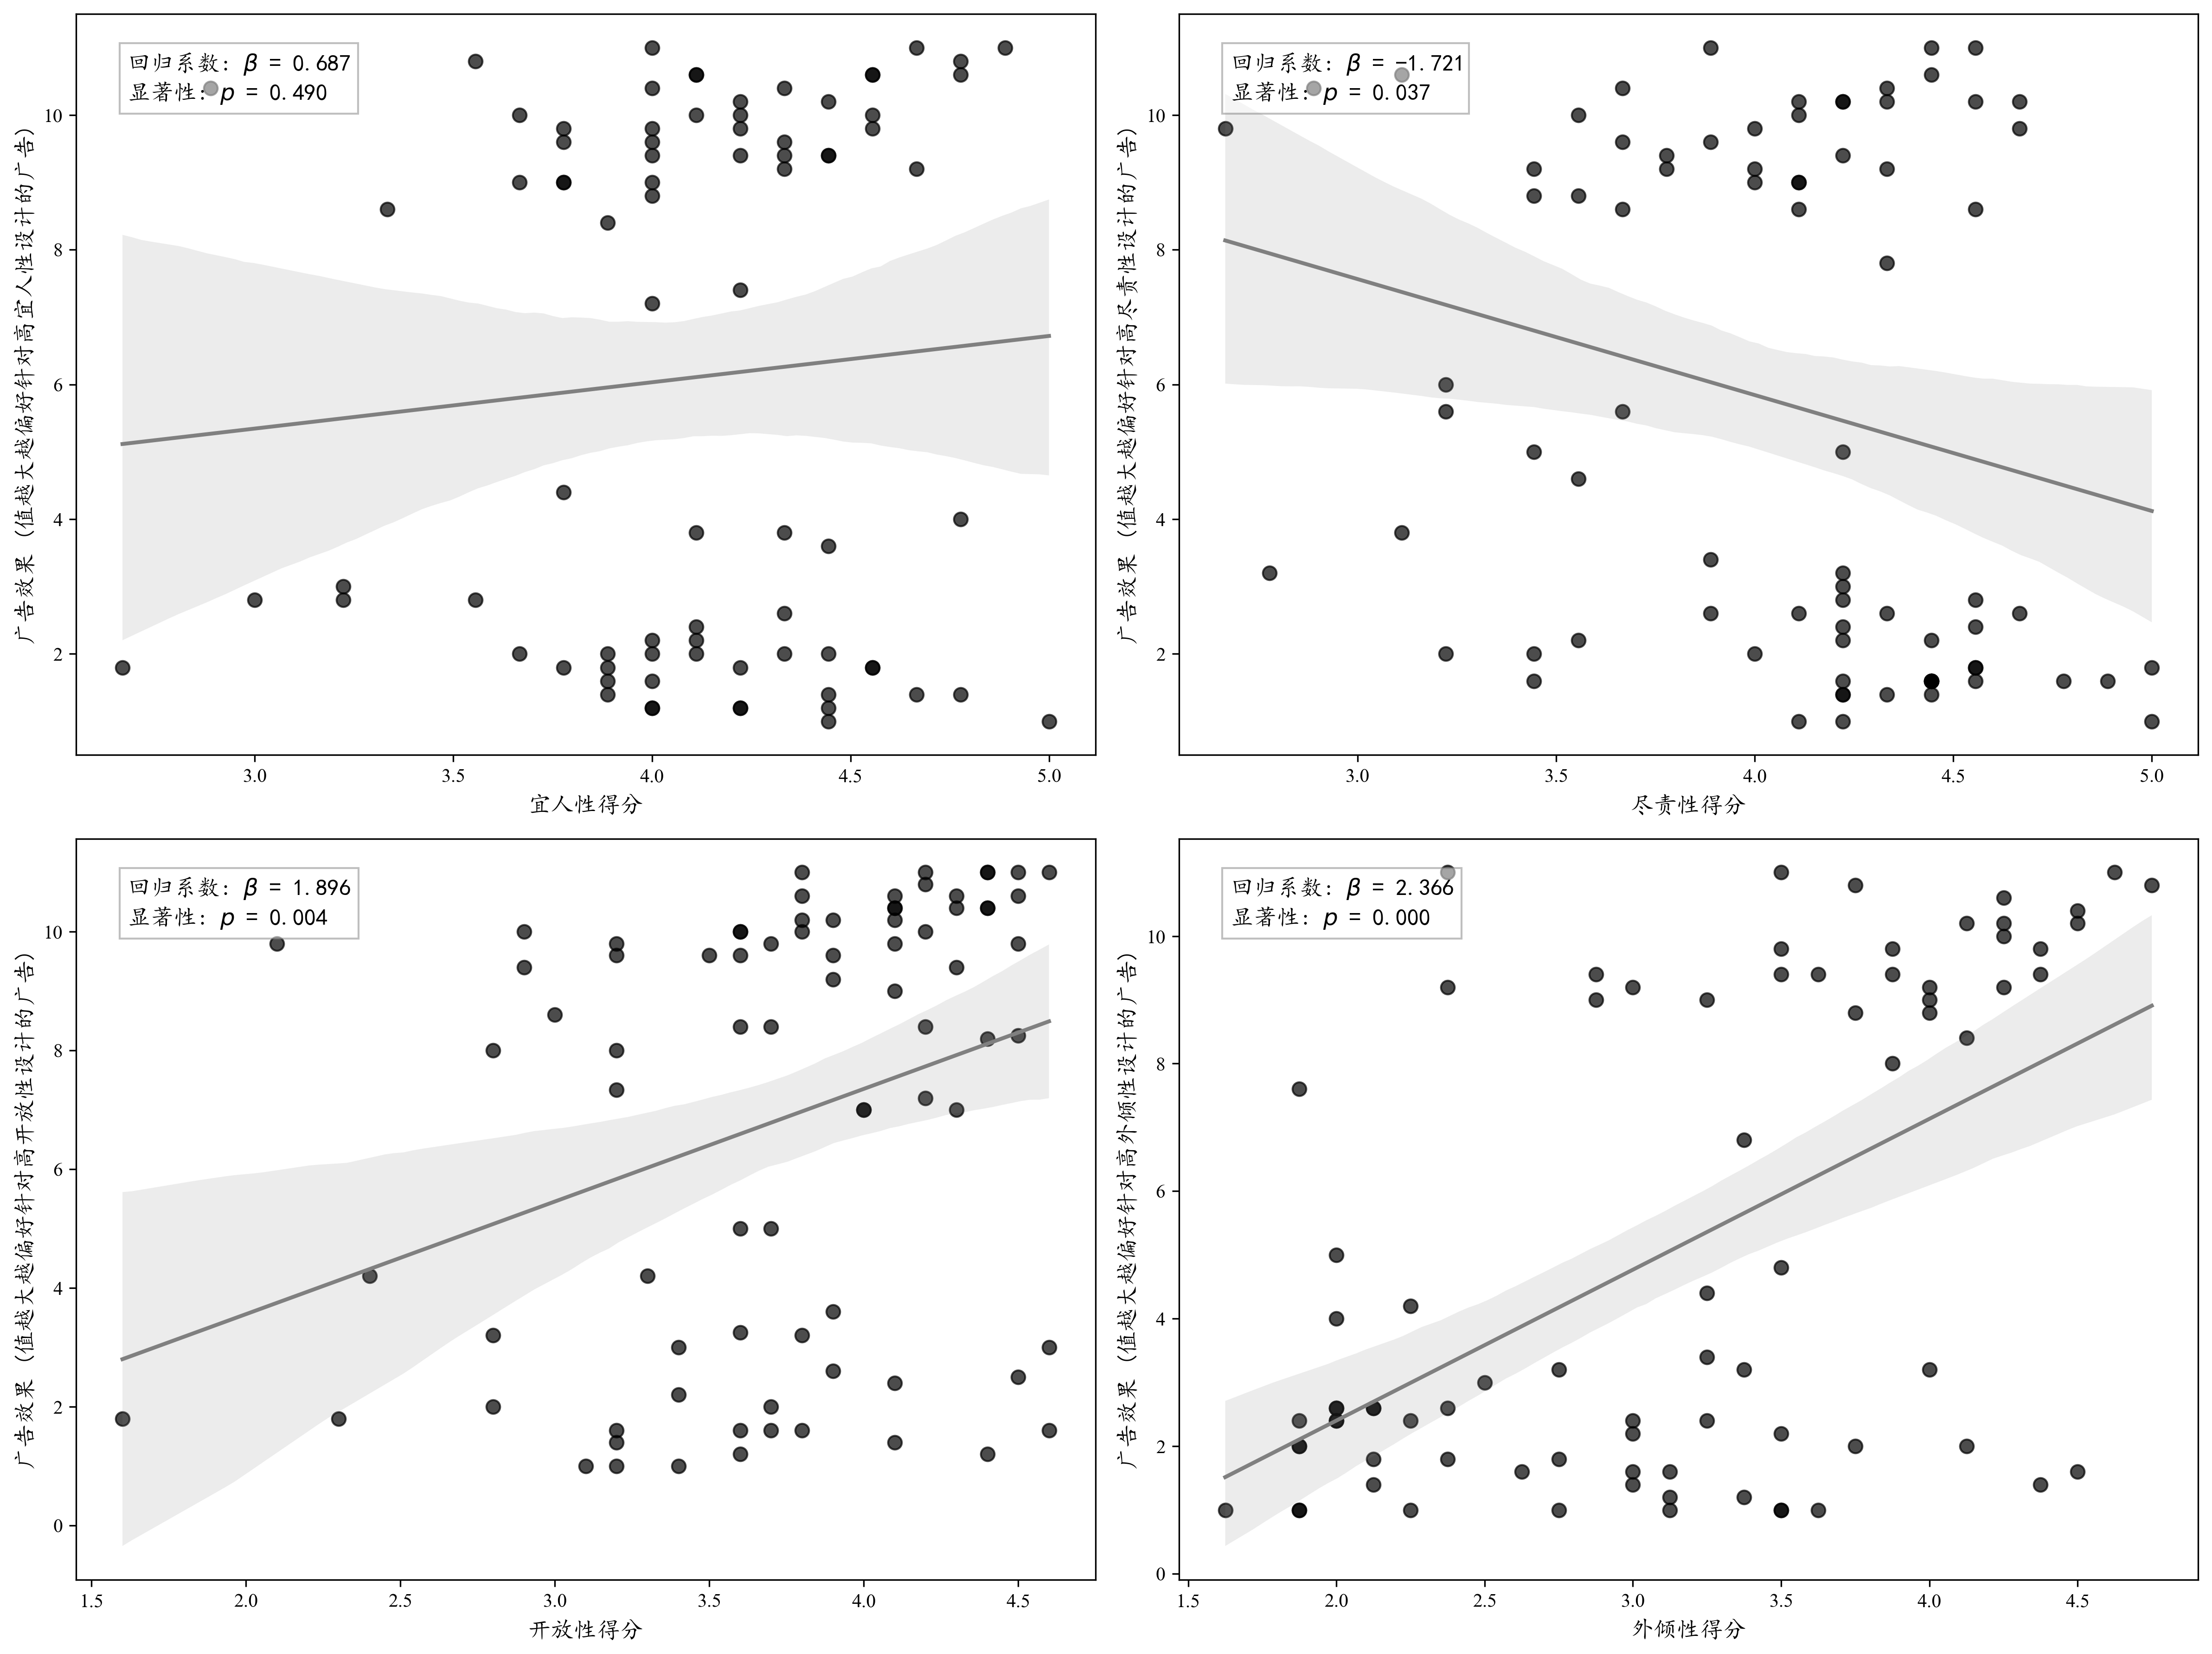
\includegraphics[width=1.0\linewidth]{Image/Study1-exp4-result.png}
    \caption{\label{fig:Study1-exp4-result}四个人格特质对相应广告效果评分的影响(含95\%置信区间)}
\end{figure}

与实验3相同,为进一步探讨参与者偏好个性化广告的原因,我们通过参与者选择的吸引他们的关键词进行分析。对于回归分析中个性化效果显著的开放性和外倾性维度,关键词特征分析结果与个性化设计方向一致。

如表\ref{tab:openness_product_preference}所示,在开放性维度上,高开放性个体偏好的Top关键词包括“无畏创新”(70.45%)、“创意P图”(45.45%)和“探索未知”(43.18%),这些词语正是针对高开放性设计时突出的特征。而低开放性个体偏好的Top关键词为“抗衰耐用”(44.44%)、“简单又可靠”(38.89%)和“创意P图功能”(36.11%),其中前两个词语是针对低开放性设计的特征,而“创意P图功能”则是广告中常见的功能性亮点,因此受到不同类型个体的广泛关注。

如表\ref{tab:extraversion_product_preference}所示,在外倾性维度上,高外倾性个体偏好的Top关键词包括“颜值在线”(36.59\%)、“出场都是焦点”(26.83\%)和“全场瞩目必备”(17.07\%),这些词语明显强调了外倾性个体关注的社交形象和外在表现,与高外倾性个性化设计一致。而低外倾性个体偏好的Top关键词前三位主要为功能性词语,接下来的关键词“无干扰”(23.08\%)、“助力你的个人空间”(23.08\%)和“安静中自由天地”(20.51\%)则与低外倾性特质匹配,突出其对安静和隐私的需求。

对于个性化效果未达到显著水平的宜人性维度(表 \ref{tab:agreeableness_product_preference}),结果呈现出有趣的现象。关键词“充满理解与关怀”(针对高宜人设计,44.44\%)更多被低宜人性个体选择(48.57\%),而“真诚相待”这一针对高宜人设计的词语在低宜人性个体中排名最高(28.57\%)。这表明,在宜人性维度上,个性化设计未能显著区分高低宜人性个体的偏好,可能是由于高低宜人性个体在广告偏好上的差异较小。

对于回归结果呈现负向个性化效果的尽责性维度(表 \ref{tab:conscientiousness_product_preference}),关键词分析结果进一步揭示了这一现象背后的可能原因。一些针对低尽责性设计的关键词,如“简单享受”和“随性而为”,在高尽责性个体中反而被频繁选择,表明这些词语对高尽责性个体也具有吸引力。此外,针对高尽责性设计的关键词,如“100\%信号强度”和“每个细节都完美无瑕”,在低尽责性个体中更受欢迎。这一结果与实验3类似,可能是由于这些词语与开放性特质存在一定的关联性,导致高开放性个体在高尽责性组中对这些词语表现出偏好。

此外,为进一步理解实验中尽责性和宜人性维度未能呈现预期效果的原因,我们参考了先前研究中收集的5110名参与者的人格数据分布(图\ref{fig:Study1-exp4-distribution})。比较发现,本研究中(浅色)宜人性和尽责性维度的分布在高分段聚集了更多被试,这意味着我们的样本中高尽责性和高宜人性个体的比例较高。这一分布特性可能导致偏好上的内部差异性被放大,从而影响了高低水平组的区分效果。例如,在尽责性维度上,高水平组中可能包含了一些具有高开放性特质的个体,而开放性与“简单享受”“随性而为”等词语高度相关,因此这些词语即使针对低尽责性设计,也会被部分高尽责性个体偏好。同样,在宜人性维度上,高水平组内部可能存在更多异质性,导致高宜人性个体未能表现出一致的偏好。因此,数据分布的偏向性可能是导致尽责性和宜人性维度个性化效果未达预期的重要原因。这一结果提示未来研究在划分高低水平组时,应结合更大规模的标准化样本进行比较,或采用连续性指标而非简单的中位数划分,以提高高低水平组的区分精度,进而更准确地检验个性化广告效果。

\begin{table}[H]
    \centering
    \caption{\label{tab:agreeableness_product_preference} 高宜人个体与低宜人个体广告词偏好}
    {\tablesongti % 整个表格环境应用宋体六号字体
    \renewcommand{\arraystretch}{1} % 调整行距
    \begin{tabularx}{\linewidth}{>{\raggedright\arraybackslash}X c >{\raggedright\arraybackslash}X c}
        \toprule
        \textbf{高宜人个体} & \textbf{比例} & \textbf{低宜人个体} & \textbf{比例} \\
        \midrule
        \textcolor{darkgreen}{充满理解与关怀} & \textcolor{darkgreen}{44.44\%} & 充满理解与关怀 & 48.57\% \\
        \textcolor{darkgreen}{用心沟通} & \textcolor{darkgreen}{35.56\%} & \textcolor{red}{AI防窥功能} & \textcolor{red}{31.43\%} \\
        \textcolor{darkgreen}{真诚相待} & \textcolor{darkgreen}{35.56\%} & 真诚相待 & 28.57\% \\
        \textcolor{darkgreen}{不惧真我} & \textcolor{darkgreen}{31.11\%} & \textcolor{red}{保护你的隐私} & \textcolor{red}{28.57\%} \\
        AI防窥功能 & 28.89\% & \textcolor{red}{敢于直言} & \textcolor{red}{25.71\%} \\
        实时AI翻译功能 & 22.22\% & 实时AI翻译功能 & 22.86\% \\
        敢于直言 & 17.78\% & \textcolor{red}{独立自主} & \textcolor{red}{22.86\%} \\
        \textcolor{darkgreen}{保护你的隐私} & \textcolor{darkgreen}{15.56\%} & \textcolor{red}{不惧真我} & \textcolor{red}{20.00\%} \\
        独立自主 & 15.56\% & 用心沟通 & 20.00\% \\
        \textcolor{darkgreen}{温暖科技} & \textcolor{darkgreen}{13.33\%} & 温暖科技 & 11.43\% \\
        \textcolor{darkgreen}{只属于你自己} & \textcolor{darkgreen}{8.89\%} & \textcolor{red}{只属于你自己} & \textcolor{red}{11.43\%} \\
        \bottomrule
    \end{tabularx}
    \vspace{0.1mm}
    \caption*{\raggedright \footnotesize 注:绿色为针对高宜人设计的词语特征,红色为针对低宜人设计的词语特征。}
    }
\end{table}


\begin{table}[H]
    \centering
    \caption{\label{tab:openness_product_preference} 高开放个体与低开放个体广告词偏好}
    {\tablesongti % 整个表格环境应用宋体六号字体
    \renewcommand{\arraystretch}{1} % 调整行距
    \begin{tabularx}{\linewidth}{>{\raggedright\arraybackslash}X c >{\raggedright\arraybackslash}X c}
        \toprule
        \textbf{高开放个体} & \textbf{比例} & \textbf{低开放个体} & \textbf{比例} \\
        \midrule
        \textcolor{darkgreen}{无畏创新} & \textcolor{darkgreen}{70.45\%} & \textcolor{red}{抗摔耐用} & \textcolor{red}{44.44\%} \\
        \textcolor{darkgreen}{创意P图功能} & \textcolor{darkgreen}{45.45\%} & \textcolor{red}{简单又可靠} & \textcolor{red}{38.89\%} \\
        \textcolor{darkgreen}{探索未知} & \textcolor{darkgreen}{43.18\%} & 创意P图功能 & 36.11\% \\
        AI识别 & 22.73\% & AI识别 & 33.33\% \\
        \textcolor{darkgreen}{创意无限} & \textcolor{darkgreen}{20.45\%} & \textcolor{red}{熟悉的经典} & \textcolor{red}{30.56\%} \\
        \textcolor{darkgreen}{激发你的每一个创新想法} & \textcolor{darkgreen}{15.91\%} & 无畏创新 & 27.78\% \\
        \textcolor{darkgreen}{抗摔耐用} & \textcolor{darkgreen}{13.64\%} & \textcolor{red}{让生活更省心} & \textcolor{red}{19.44\%} \\
        简单又可靠 & 13.64\% & 探索未知 & 16.67\% \\
        让生活更省心 & 9.09\% & \textcolor{red}{稳定生活好选择} & \textcolor{red}{11.11\%} \\
        熟悉的经典 & 9.09\% & 轻松应对 & 8.33\% \\
        性能提升 & 6.82\% & 创意无限 & 5.56\% \\
        轻松应对 & 4.55\% & 性能提升 & 5.56\% \\
        & & 每一天的琐碎小事 & 2.78\% \\
        & & 激发你的每一个创新想法 & 2.78\% \\
        \bottomrule
    \end{tabularx}
    \vspace{0.1mm}
    \caption*{\raggedright \footnotesize 注:绿色为针对高开放设计的词语特征,红色为针对低开放设计的词语特征。}
    }
\end{table}

\begin{table}[H]
    \centering
    \caption{\label{tab:extraversion_product_preference} 高外倾个体与低外倾个体广告词偏好}
    {\tablesongti % 整个表格环境应用宋体六号字体
    \renewcommand{\arraystretch}{1} % 调整行距
    \begin{tabularx}{\linewidth}{>{\raggedright\arraybackslash}X c >{\raggedright\arraybackslash}X c}
        \toprule
        \textbf{高外倾个体} & \textbf{比例} & \textbf{低外倾个体} & \textbf{比例} \\
        \midrule
        \textcolor{darkgreen}{颜值在线} & \textcolor{darkgreen}{36.59\%} & AI P图随心创作 & 56.41\% \\
        \textcolor{darkgreen}{出场都是焦点} & \textcolor{darkgreen}{26.83\%} & 零束缚 & 30.77\% \\
        AI P图随心创作 & 26.83\% & 强悍性能 & 28.21\% \\
        无干扰 & 17.07\% & \textcolor{red}{无干扰} & \textcolor{red}{23.08\%} \\
        \textcolor{darkgreen}{全场瞩目必备} & \textcolor{darkgreen}{17.07\%} & \textcolor{red}{助力你的个人空间} & \textcolor{red}{23.08\%} \\
        \textcolor{darkgreen}{让你的社交不再有障碍} & \textcolor{darkgreen}{14.63\%} & 随时捕捉灵感 & 23.08\% \\
        零束缚 & 14.63\% & \textcolor{red}{让你沉浸在属于自己的世界} & \textcolor{red}{20.51\%} \\
        开放式AI翻译 & 12.20\% & \textcolor{red}{安静中自有天地} & \textcolor{red}{20.51\%} \\
        随时捕捉灵感 & 7.32\% & 独处的美好 & 12.82\% \\
        \textcolor{darkgreen}{社交达人首选} & \textcolor{darkgreen}{7.32\%} & 让你的社交不再有障碍 & 7.69\% \\
        强悍性能 & 7.32\% & 开放式AI翻译 & 5.13\% \\
        助力你的个人空间 & 7.32\% & 颜值在线 & 2.56\% \\
        独处的美好 & 4.88\% & 出场都是焦点 & 2.56\% \\
        \textcolor{darkgreen}{让你沉浸在属于自己的世界} & \textcolor{darkgreen}{4.88\%} & 社交达人首选 & 2.56\% \\
        & & 全场瞩目必备 & 2.56\% \\
        \bottomrule
    \end{tabularx}
    \vspace{0.1mm}
    \caption*{\raggedright \footnotesize 注:绿色为针对高外倾设计的词语特征,红色为针对低外倾设计的词语特征。}
    }
\end{table}

\begin{table}[H]
    \centering
    \caption{\label{tab:conscientiousness_product_preference} 高尽责个体与低尽责个体广告词偏好}
    {\tablesongti % 整个表格环境应用宋体六号字体
    \renewcommand{\arraystretch}{1} % 调整行距
    \begin{tabularx}{\linewidth}{>{\raggedright\arraybackslash}X c >{\raggedright\arraybackslash}X c}
        \toprule
        \textbf{高尽责个体} & \textbf{比例} & \textbf{低尽责个体} & \textbf{比例} \\
        \midrule
        简单享受 & 47.62\% & 100\%信号强度 & 44.74\% \\
        便捷的AI功能 & 28.57\% & 每个细节都完美无瑕 & 42.11\% \\
        随性而为 & 26.19\% & 40\%性能提升 & 39.47\% \\
        \textcolor{darkgreen}{100\%信号强度} & \textcolor{darkgreen}{26.19\%} & 为追求卓越而生 & 28.95\% \\
        \textcolor{darkgreen}{每个细节都完美无瑕} & \textcolor{darkgreen}{23.81\%} & 强悍性能 & 26.32\% \\
        \textcolor{darkgreen}{强悍性能} & \textcolor{darkgreen}{21.43\%} & \textcolor{red}{简单享受} & \textcolor{red}{26.32\%} \\
        \textcolor{darkgreen}{40\%性能提升} & \textcolor{darkgreen}{21.43\%} & 便捷的AI功能 & 21.05\% \\
        \textcolor{darkgreen}{为追求卓越而生} & \textcolor{darkgreen}{14.29\%} & \textcolor{red}{随性而为} & \textcolor{red}{15.79\%} \\
        随时随地 & 11.90\% & \textcolor{red}{轻松生活} & \textcolor{red}{15.79\%} \\
        想怎么用就怎么用 & 9.52\% & \textcolor{red}{随时随地} & \textcolor{red}{10.53\%} \\
        轻松生活 & 9.52\% & 专业人士 & 7.89\% \\
        \textcolor{darkgreen}{专业人士} & \textcolor{darkgreen}{4.76\%} & \textcolor{red}{想怎么用就怎么用} & \textcolor{red}{2.63\%} \\
        \bottomrule
    \end{tabularx}
    \vspace{0.1mm}
    \caption*{\raggedright \footnotesize 注:绿色为针对高尽责设计的词语特征,红色为针对低尽责设计的词语特征。}
    }
\end{table}


\begin{figure}[H]
    \centering
    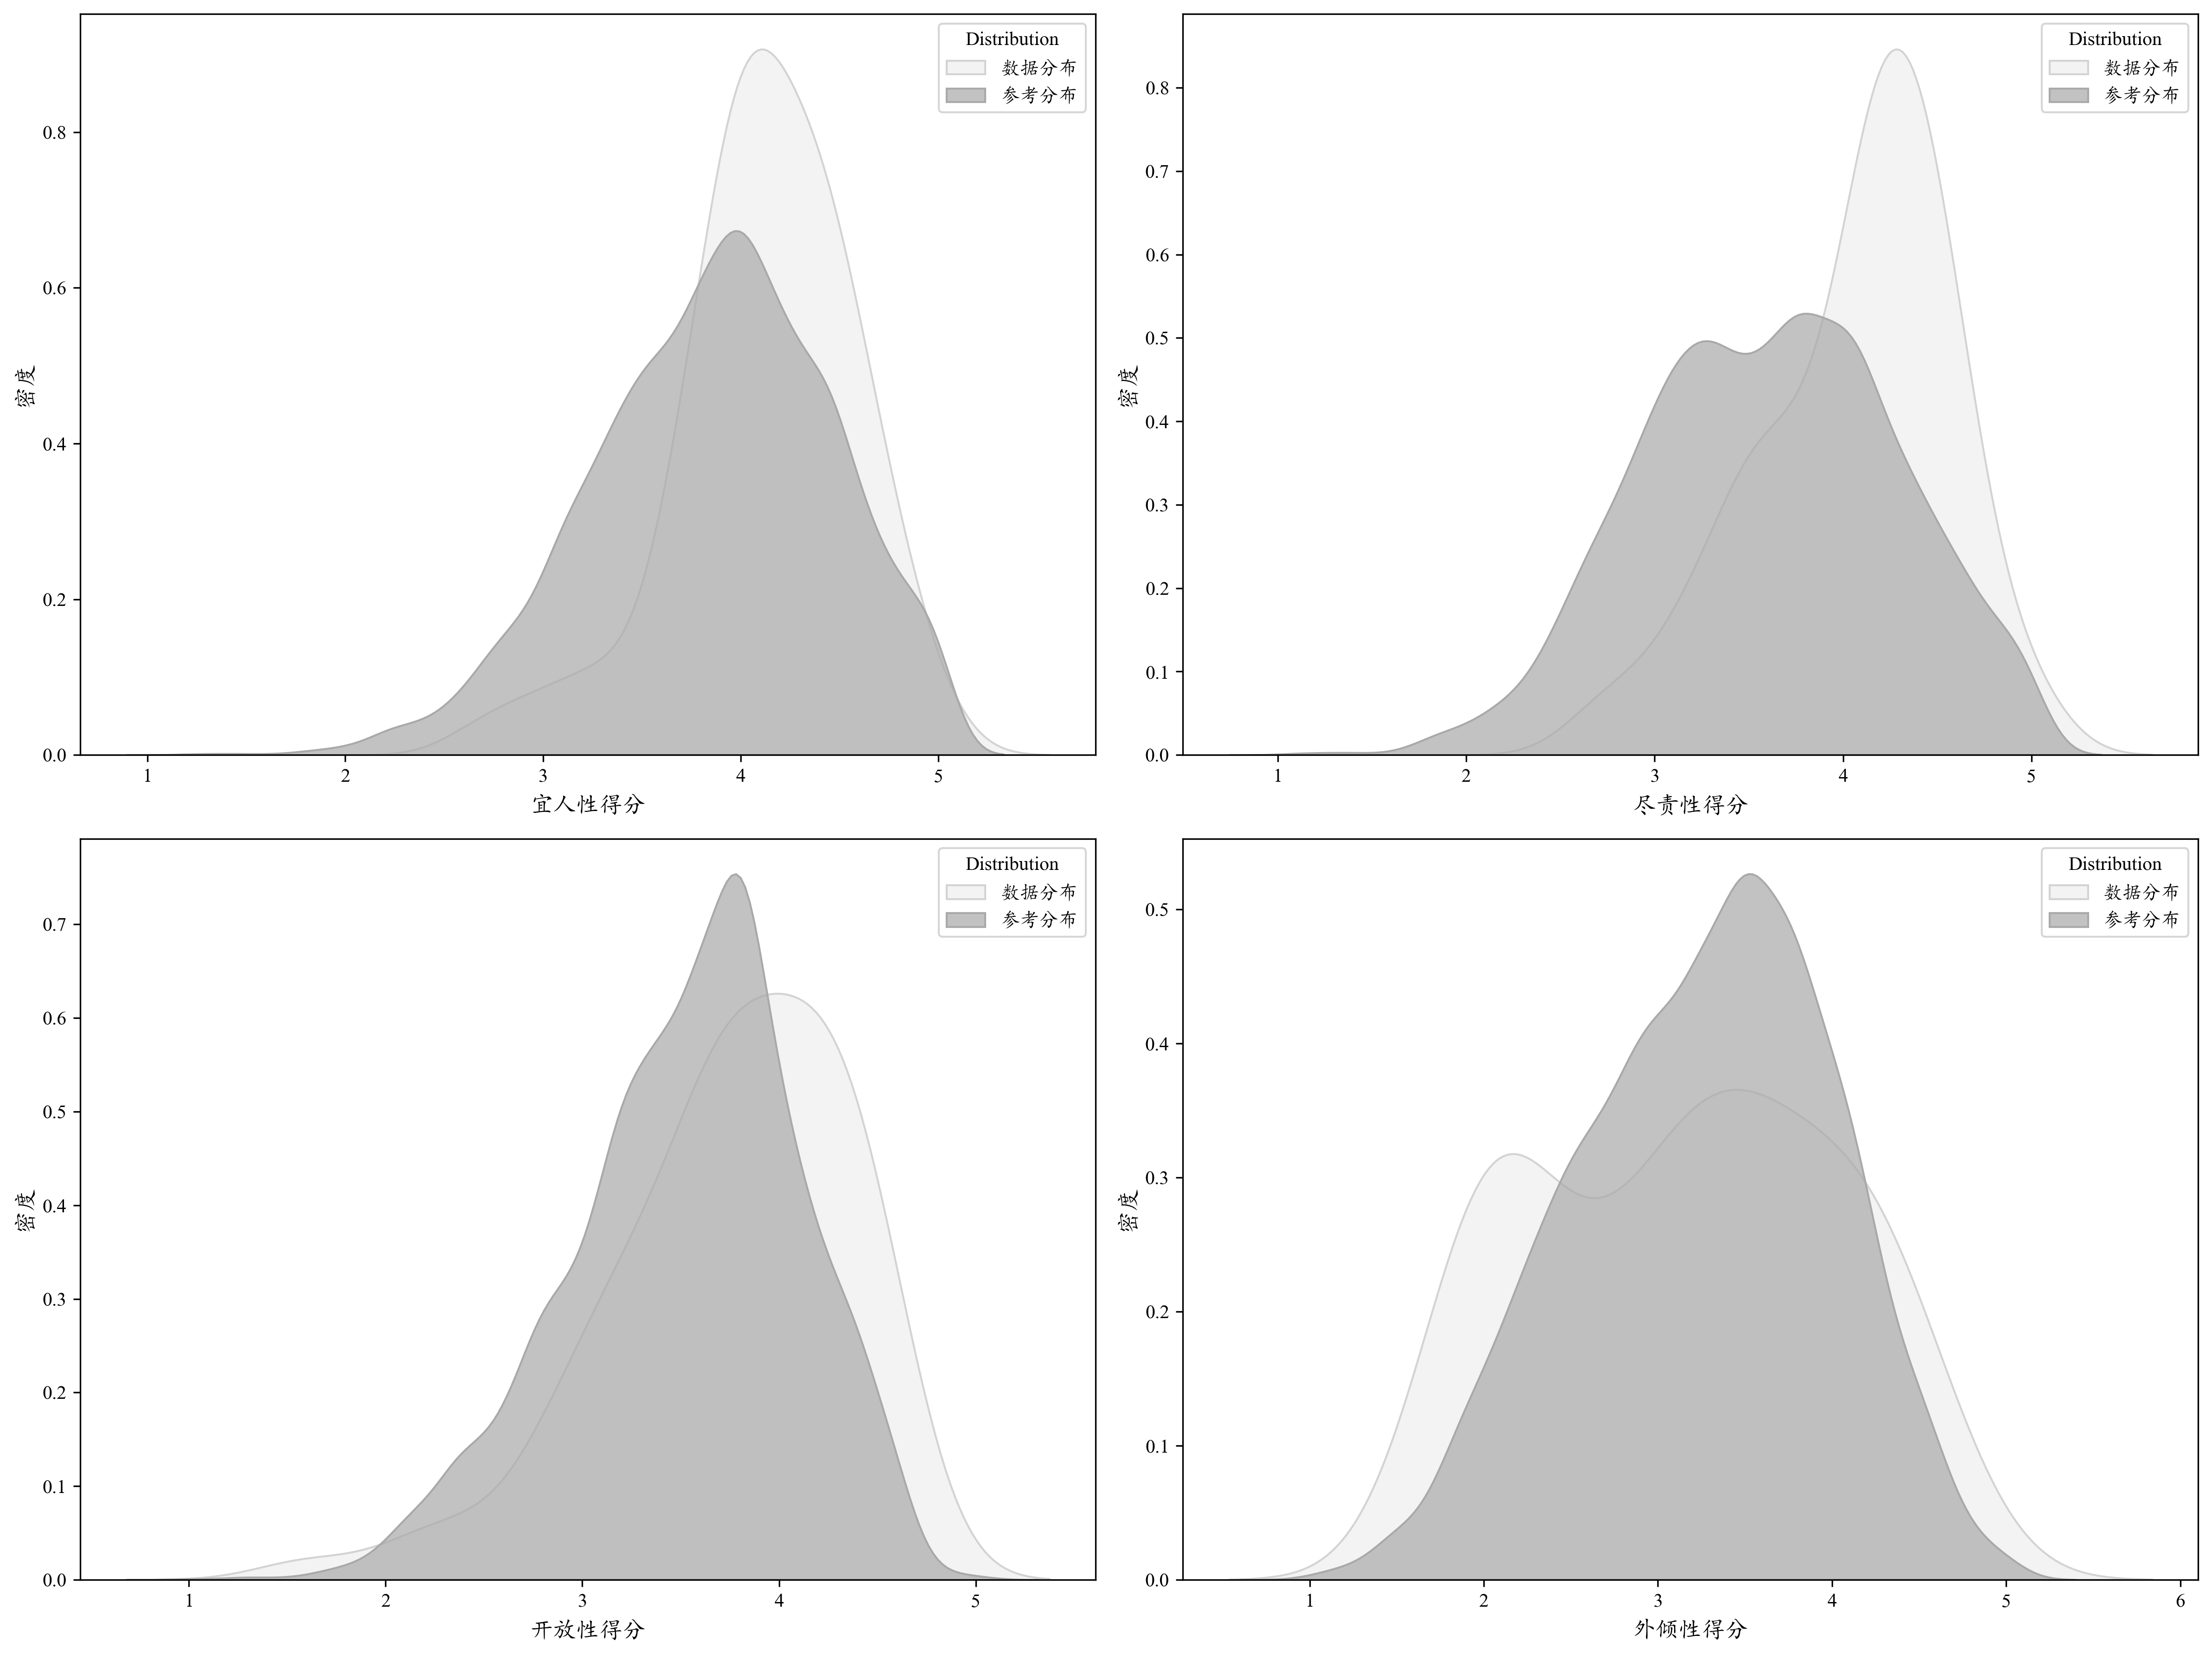
\includegraphics[width=1.0\linewidth]{Image/Study1-exp4-distribution.png}
    \caption{\label{fig:Study1-exp4-distribution}本研究与大样本数据(5110份)的人格特质分布比较}
\end{figure}

